%%%%%%%%%%%%%%%%%%%%%%%
\section{Expression fonctionnelle du besoin}
%%%%%%%%%%%%%%%%%%%%%%%

\subsection{Présentation générale}

L'objectif est de concevoir et de développer l'architecture logicielle du superviseur afin d'assurer le fonctionnement de la plate-forme. Les fonctions attendues sont :
\begin{enumerate}
	\item Assurer la communication entre le moniteur et le superviseur.
	\item Assurer la communication entre le superviseur et le robot.
	\item Superviser l'état du robot.
	\item Contrôler le déplacement du robot.
	\item Contrôler et diffuser les images de la webcam.
	\item Réaliser des missions.\\
\end{enumerate}

\noindent\framebox[\textwidth]{
\begin{minipage}{0.9\textwidth}
{\bf Remarque :}  Les plateformes matérielle et logicielle ont de nouveau évoluées cette année. Les bibliothèques fournies ont été réécrites pour faciliter leur prise en main. Bien qu'elles aient été testées, elles comportent certainement des erreurs. Soyez indulgents, nous faisons de notre mieux pour fournir une plate-forme opérationnelle !\\
{\bf Si vous remarquez des erreurs, des problèmes ou des optimisations à faire, n'hésitez pas à le communiquer} (via GitHub pour en garder la trace).
\end{minipage}
}\\

  \subsection{Diagramme de contexte}

La figure~\ref{fig:contexte} présente le superviseur dans son contexte et ses interactions avec les autres composants de la plate-forme.

 \begin{figure}[htbp]
\begin{center}
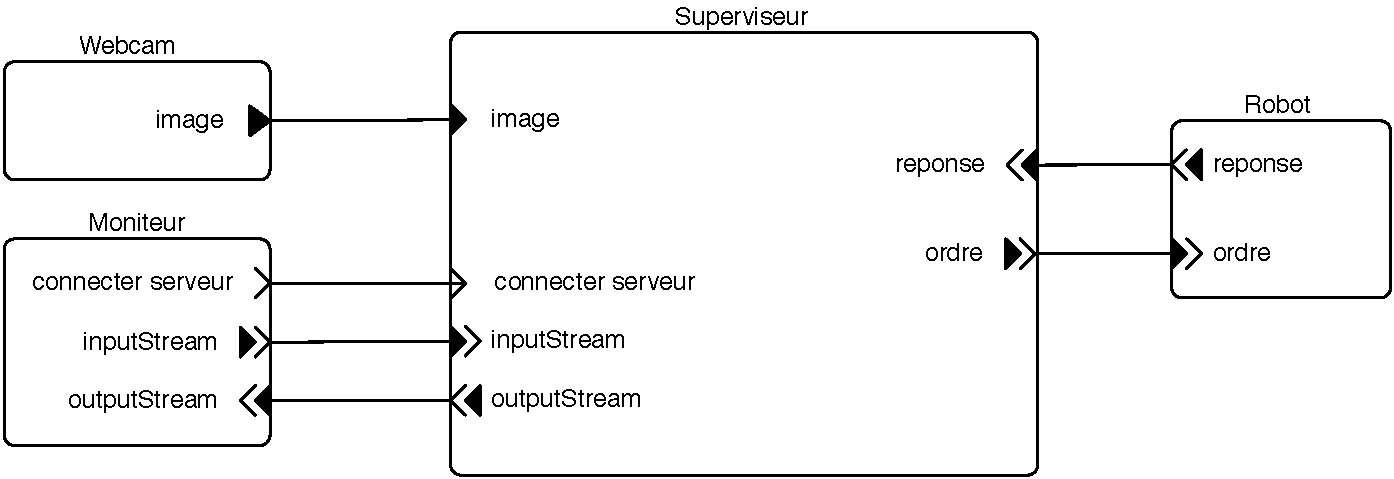
\includegraphics[scale=0.6]{figures_pdf/contexte}
\caption{Diagramme de contexte}
\label{fig:contexte}
\end{center}
\end{figure}
\FloatBarrier

La webcam produit des données (\texttt{image}) sous la forme d'un tableau d'octets. Le robot reçoit des ordres (\texttt{ordre}) sous la forme d'une chaîne de caractères et retourne une réponse aussi sous la forme d'une chaîne (\texttt{reponse}). Le moniteur envoie un événement (\texttt{connecter serveur}) pour demander la connexion avec le serveur puis établit une communication bi-directionnelle sous la forme d'un flux d'octets (\texttt{inputStream} et \texttt{outputStream}).

%Si l'on se focalise uniquement sur le superviseur, nous avons donc un unique processus (voir figure~\ref{fig:processus}).
%
% \begin{figure}[htbp]
%\begin{center}
%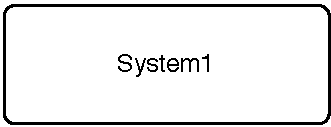
\includegraphics[scale=0.6]{figures_pdf/AADL/system}
%\caption{Vue systéme du Superviseur}
%\label{fig:processus}
%\end{center}
%\end{figure}
%\FloatBarrier


  %%%%%%%%%%%%%%%%%%%%%%%%%
\subsection{Description des fonctionnalités}
%%%%%%%%%%%%%%%%%%%%%%%%%

Vous trouverez dans cette partie la description des différentes fonctionnalités attendues. Les annexes apportent des compléments techniques.\\

\noindent\fcolorbox{black}{Fond}{%                couleur du texte, couleur du fond
\begin{minipage}{\textwidth}
L'expression des fonctionnalités est repérée par des encadrés avec un fond gris. C'est ce que vous devez réaliser.
\end{minipage}
}

%%%%%%%%%%%%%%%%%%%%%%%%%
\subsubsection{Fonctionnement du moniteur}
%%%%%%%%%%%%%%%%%%%%%%%%%

Le moniteur sert pour le contrôle du robot et la visualisation d'une scène. La communication entre le moniteur et le superviseur est réalisée par un socket avec un serveur du côté du superviseur. La communication est bi-directionnelle : le moniteur peut envoyer des requêtes et le superviseur peut envoyer des données pour mettre à jour certains éléments de l'interface. Les messages sont prédéfinis et sont présentés dans l'annexe~\ref{sec:comm_mon_sup}.


%%%%%%%%%%%%%%%%%%%%%%%%%
  \subsubsection{Communication entre le superviseur et le moniteur}
%%%%%%%%%%%%%%%%%%%%%%%%%

La communication entre le serveur et le superviseur est réalisée à l'aide d'un socket. Le superviseur joue le rôle de serveur. Toutes les fonctions pour gérer la communication entre le moniteur et le superviseur sont fournies dans {\tt monitor}.

Les figures~\ref{fig:diag1_2} et~\ref{fig:diag3_6}  illustrent le mode de fonctionnement nominal attendu pour la communication entre le superviseur et le moniteur.

%https://sequencediagram.org

%%%%%%%%%%%%%%%%%%%%%%%%%
\paragraph{Lancement du serveur.} Le lancement du serveur est réalisé à l'aide de la méthode {\tt Open} de la classe {\tt ComMonitor}.\\

\req{Le lancement du serveur doit être réalisé au démarrage du superviseur. En cas d'échec du démarrage du serveur, un message textuel doit être  affiché sur la console de lancement de l'application. Ce message doit signaler le problème et le superviseur doit s'arrêter.}


%%%%%%%%%%%%%%%%%%%%%%%%%
\paragraph{Etablissement du socket.} La connexion entre le moniteur et le superviseur est réalisée suite à la demande de l'utilisateur via l'interface graphique. Lorsque la demande est faite, un socket est créé, il faut donc que le serveur soit en attente d'une demande de connexion, c'est-à-dire que la méthode {\tt AcceptClient} de la classe {\tt ComMonitor} soit en cours d'exécution. Cette méthode est bloquante.\\

\req{La connexion entre le moniteur et le superviseur (via le socket) doit être établie suite à la demande de connexion de l'utilisateur.}

%Terminal->*Supervisor:exec
%note left of Supervisor:  (req 1) start server
%Supervisor->+Supervisor: ComMonitor::Open()
%Supervisor-->-Supervisor:err
%alt err != failed 
%    Supervisor->+Supervisor: ComMonitor::AcceptClient()
%    Monitor->Supervisor: connexion
%    note left of Supervisor:  (req 2) connect socket
%    Supervisor->Monitor:accept
%    Supervisor-->-Supervisor:err
%    
%else
%    Supervisor->Terminal: print("server failed")
%    destroy Supervisor
%end
\begin{figure}[htbp]
\begin{center}
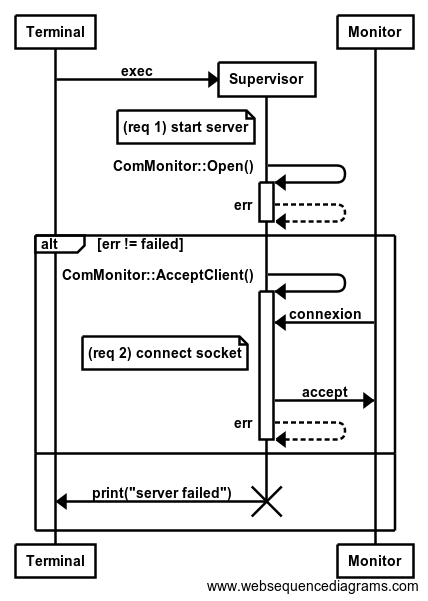
\includegraphics[scale=0.4]{./seq_req/req1-2}
\caption{Diagramme de séquence des fonctionnalités 1 à 2}
\label{fig:diag1_2}
\end{center}
\end{figure}

%%%%%%%%%%%%%%%%%%%%%%%%%
\paragraph{Réception des messages.} La réception des messages du serveur par le superviseur est réalisée par l'appel de la méthode  {\tt Read} de la classe {\tt ComMonitor}. Cette méthode est bloquante. Les messages du moniteur vers le superviseur sont pré-formatés dans la classe {\tt Message} et définis dans l'annexe~\ref{sec:mts}.\\

\req{Tous les messages envoyés depuis le moniteur doivent être réceptionnés par le superviseur.}


%%%%%%%%%%%%%%%%%%%%%%%%%
\paragraph{Envoi des messages.} L'envoi des messages du superviseur vers le moniteur est réalisé à l'aide de la fonction {\tt Write} de la classe {\tt ComMonitor}. Les messages du superviseur vers le moniteur sont pré-formatés et définis dans l'annexe~\ref{sec:stm}.\\

\req{L'application superviseur doit être capable d'envoyer les messages au moniteur (via le serveur) avec un délai d'au plus 10~ms.}

%%%%%%%%%%%%%%%%%%%%%%%%%
\paragraph{Détection de la perte de communication.} La perte de communication entre le moniteur et le superviseur est détectée lors de la lecture sur le socket. La méthode {\tt Read} retourne un message de type {\tt MESSAGE\_MONITOR\_LOST}  si la communication est perdue. \\

\req{Le superviseur doit détecter la perte de communication avec le moniteur. En cas de perte de la communication un message doit être affiché sur la console de lancement du superviseur.}

%%%%%%%%%%%%%%%%%%%%%%%%%
\paragraph{Reprise de la communication.}  La communication entre le moniteur et le superviseur est fermé à l'aide de la méthode {\tt Close} de la classe {\tt ComMonitor}. {\bf Attention} cette fonctionnalité ne peut être mise en place que lorsque l'ensemble de l'application est déjà réalisée, il ne sert à rien d'y travailler tant que le reste n'est pas fait.\\

\req{En cas de perte de communication entre le superviseur et moniteur, il faut stopper le robot,  la communication avec le robot, fermer le serveur et déconnecter la caméra afin de revenir dans le même état qu'au démarrage du superviseur.}

%loop message is not MESSAGE_MONITOR_LOST
%par
%note left of Monitor: (req 3) receive message from Monitor
%Supervisor->+Supervisor: ComMonitor::Read()
%Monitor->Supervisor: message
%Supervisor-->-Supervisor: message
%note over Supervisor: compute message
%else
%note left of Monitor: (req 4) send message to Monitor
%note over Supervisor: wait message to send
%Supervisor->Monitor: ComMonitor::Write(message)
%end
%note left of Monitor
%    (req 5) detect loss of 
%    communication between Supervisor
%    and Monitor
%end note
%end
%note right of Supervisor: (req 6) kill server
%Supervisor->+Supervisor:ComMonitor::Close
%Supervisor->Terminal:print("Monitor is lost")
%note over Supervisor: clear Supervisor
\begin{figure}[htbp]
\begin{center}
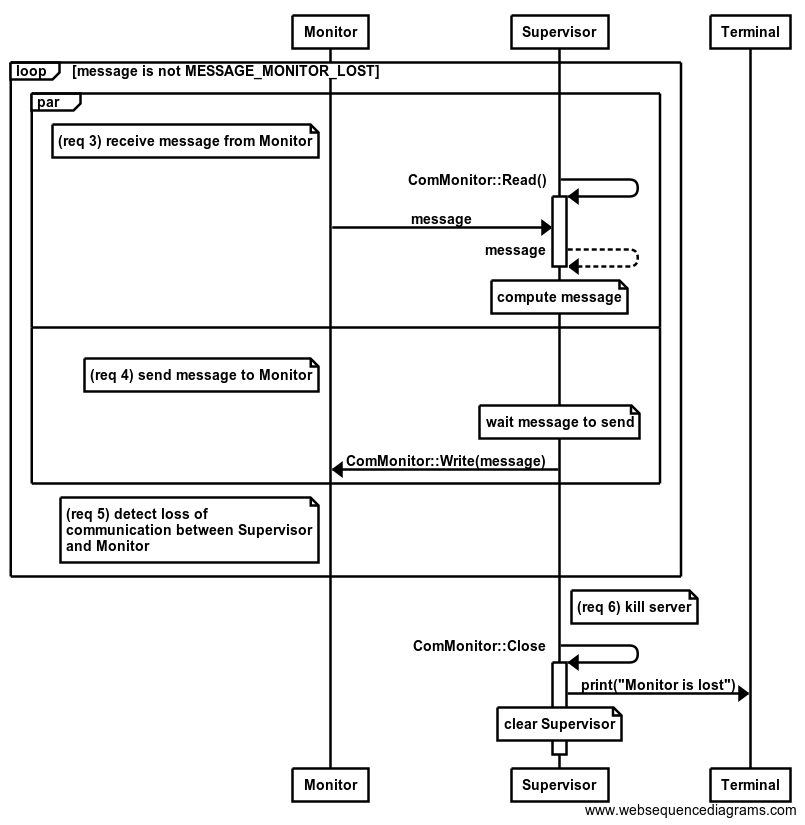
\includegraphics[scale=0.4]{./seq_req/req3-6}
\caption{Diagramme de séquence des fonctionnalités 3 à 6}
\label{fig:diag3_6}
\end{center}
\end{figure}
\FloatBarrier

 %%%%%%%%%%%%%%%%%%%%%%%%%
\subsubsection{Communication entre le superviseur et le robot}
%%%%%%%%%%%%%%%%%%%%%%%%%

La communication avec le robot s'effectue par le biais d'émetteur-récepteur Xbee. Pour communiquer, il est nécessaire de commencer par ouvrir la communication entre le superviseur et le boîtier Xbee. Toutes les fonctions de gestion de la communication entre le robot et le superviseur sont fournies dans la bibliothèque {\tt robot}. La figure~\ref{fig:diag7_9} illustre les fonctionnalités 7 à 9.

\paragraph{Mettre en place la communication avec le robot.} L'ouverture de la communication (c'est-à-dire la réservation d'un port série) avec le robot se fait à l'aide de la fonction {\tt Open} de la classe {\tt ComRobot}. Cette demande est automatiquement demandée par le moniteur dès que le socket est en place.\\

\req{Dès que la communication avec le moniteur est en place, la communication entre le superviseur et le robot doit être ouverte. Si la communication est active, il faut envoyer un message d'acquittement au moniteur. En cas d'échec, un message le signalant est renvoyé au moniteur.}

\paragraph{Surveillance de la communication avec le robot.} La communication entre le robot et le superviseur peut être perdue. Afin de surveiller cela, il faut mettre en place un mécanisme permettant d'inférer cette perte. L'envoi des messages au robot se fait à l'aide de la fonction {\tt Write} de la classe {\tt ComRobot}. En cas d'échec de communication, la méthode retourne un message contenant un code d'erreur. Cependant, l'envoi d'un message par Xbee peut retourner un échec même si le médium de communication est encore opérationnel.

De ce fait, le simple retour d'un échec ne suffit pas à déterminer si la communication est définitivement perdue ou bien si c'est une erreur fugace. Afin de conclure que la communication est perdue, il faut donc mettre en place un mécanisme de compteur. Pour cela, il faut incrémenter un compteur à chaque échec sur l'envoi d'un message et le remettre à zéro à chaque succès. Si le compteur dépasse 3, la communication est alors déclarée perdue.\\

\req{La communication entre le robot et le superviseur doit être surveillée par un mécanisme de compteur afin de détecter une perte du médium de communication.}

\paragraph{Perte de la communication avec le robot.} Le medium de communication entre le robot et le superviseur est stoppé par l'appel à la fonction {\tt close\_communication\_robot}.\\

\req{Lorsque la communication entre le robot et le superviseur est perdue, un message spécifique doit être envoyé au moniteur. Le système doit fermer la communication entre le robot et le superviseur et se remettre dans un état initial permettant de relancer la communication.}


%%%%%%%%%%%%%%%%%%%%%%%%%
\subsubsection{Démarrage du robot}
%%%%%%%%%%%%%%%%%%%%%%%%%

Tous les messages entre le superviseur et le robot sont décrits dans l'annexe~\ref{sec:sec:comm_rob_sup}. L'envoi d'un message se fait par l'utilisation de la méthode {\tt Write} de la classe {\tt ComRobot}. La figure~\ref{fig:diag10_11} représente la séquence pour les fonctionnalités 10 et 11.\\

\noindent\framebox[\textwidth]{
\begin{minipage}{0.9\textwidth}
{\bf Remarque :}  Aucun mécanisme n'est mis en {\oe}uvre dans l'implémentation de {\tt Write} de {\tt ComRobot} pour se prémunir des appels concurrents.
\end{minipage}
}


%%%%%%%%%%%%%%%%
\paragraph{Démarrage sans watchdog du robot.} Le robot a deux modes de démarrage. Un mode simple, dit sans watchdog et un mode évolué exposé ci-après.\\

\req{Lorsque l'utilisateur demande, via le moniteur, le démarrage sans watchdog, le robot doit démarrer dans ce mode. En cas de succès, un message d'acquittement est retourné au moniteur. En cas d'échec, un message indiquant l'échec est transmis au moniteur.}


%note right of Monitor: (req 7) connect robot
%Monitor->Supervisor:connexion robot
%Supervisor->+Supervisor: ComRobot::Open()
%Supervisor-->-Supervisor:err
%alt err == 0
%Supervisor->Monitor: ComMonitor::Write(ACK)
%else
%Supervisor->Monitor: ComMonitor::Write(NO_ACK)
%end
%note right of Monitor
%    (req 8) monitor communication with robot
%end note
%loop cmpt <= 3
%Supervisor->+Supervisor: ComRobot:Write(message)
%Supervisor-->-Supervisor:msg
%alt msg is not an error 
%    note over Supervisor: cmpt = 0
%else
%   note over Supervisor: cmpt ++
%end
%end
%note right of Monitor: (req 9) robot communication lost
%Supervisor->Monitor: ComMonitor::Write(LOST_DMB)
%Supervisor->Supervisor: ComRobot::Close()
%note over Supervisor: initialize_communication_robot

\begin{figure}[htbp]
\begin{center}
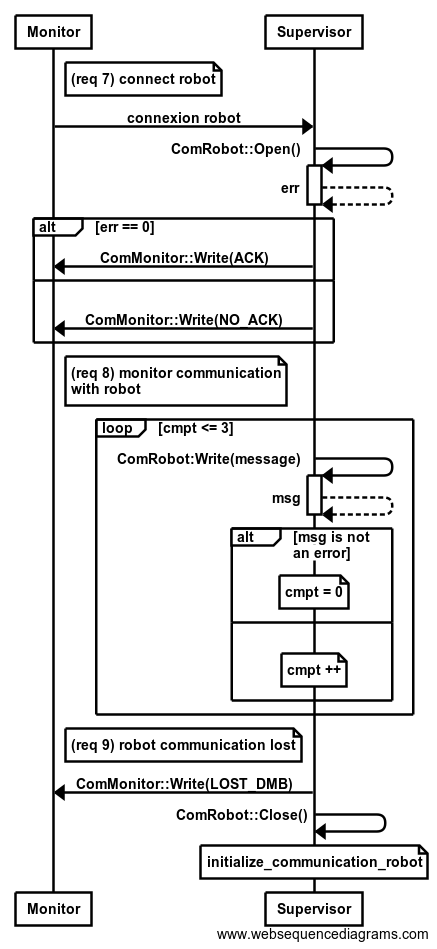
\includegraphics[scale=0.48]{./seq_req/req7-9}
\caption{Diagramme de séquence des fonctionnalités 7 à 9}
\label{fig:diag7_9}
\end{center}
\end{figure}
\FloatBarrier

%%%%%%%%%%%%%%%%
\paragraph{Démarrage avec watchdog du robot.} En cas de perte de la communication entre le superviseur et le robot, ce dernier n'est plus contrôlable et continue à exécuter des ordres. Pour éviter cela, un mécanisme de surveillance à base de watchdog a été mis en place sur le robot.

Le principe est simple : au démarrage du robot (c.-à-d. quand le robot traite l'ordre de démarrage avec watchdog), un watchdog périodique d'une seconde est lancé. \`A chaque expiration du watchdog un compteur dans le robot est incrémenté. Si le compteur atteint 3, le robot s'arrête et doit être redémarré manuellement.  Pour éviter cela, le robot doit recevoir du superviseur un ordre spécifique de rechargement du watchdog (DMB\_RELOAD\_WD). Si l'ordre est valide, le compteur est décrémenté de 1 (minimum 0). Pour que cet ordre soit valide il faut qu'il arrive au moment où le watchdog expire avec un tolérance de 50~ms. \\

\req{Lorsque l'utilisateur demande, via le moniteur, le démarrage avec watchdog, le robot doit démarrer dans ce mode. Un message d'acquittement est retourné au moniteur. En cas d'échec, un message indiquant l'échec est transmis au moniteur.

Une fois le démarrage effectué, le robot doit rester vivant. Pour cela, il faut que le moniteur envoie régulièrement le message de rechargement du watchdog.}

%alt
%note right of Monitor
%    (req 10) start without watchdog
%end note
%Monitor->Supervisor:start_robot_without_wd
%Supervisor->+Supervisor: ComRobot::Write(START_WITHOUT_WD)
%Supervisor-->-Supervisor:err
%note over Monitor, Supervisor:ack or no_ack
%
%else
%note right of Monitor
%    (req 11) start with watchdog
%end note
%
%Monitor->Supervisor:start_robot_with_wd
%Supervisor->+Supervisor: ComRobot::Write(START_WITH_WD)
%Supervisor-->-Supervisor:err
%alt err == ROBOT_OK
%Supervisor->Monitor: ComMonitor::Write(message(ACK))
%note over Supervisor
%    start to reload wd periodically
%end note
%else
%Supervisor->Monitor: ComMonitor::Write(message(NO_ACK)
%end
%end

\begin{figure}[htbp]
\begin{center}
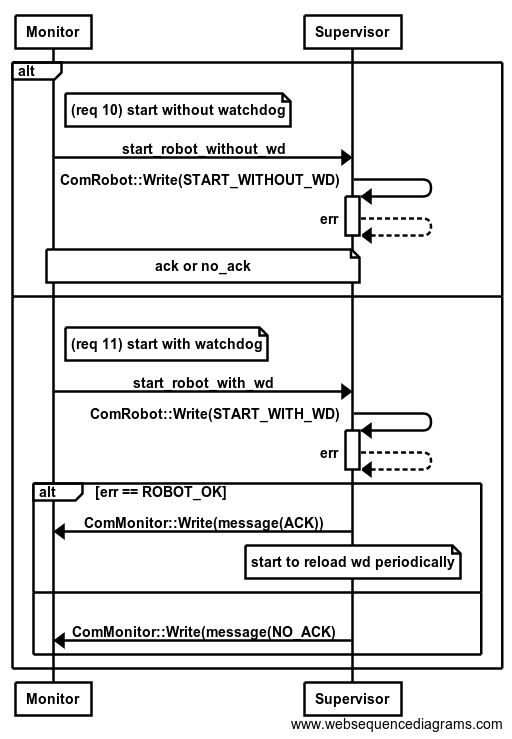
\includegraphics[scale=0.4]{./seq_req/req10-11}
\caption{Diagramme de séquence des fonctionnalités 10 et 11}
\label{fig:diag10_11}
\end{center}
\end{figure}
\FloatBarrier

%%%%%%%%%%%%%%%%%%%%%%%%%
\subsubsection{Déplacement et état du robot}
%%%%%%%%%%%%%%%%%%%%%%%%%

Le robot n'a aucune intelligence et ne réagit qu'aux ordres qu'il reçoit.  La figure~\ref{fig:diag12_13} représente la séquence pour les fonctionnalités 12 et 13.

%%%%%%%%%%%%%%%%%%%%%%%%%
\paragraph{Déplacement manuel du robot.} Le robot peut recevoir cinq ordres de mouvement (avancer, reculer, tourner à droite, tourner à gauche et stopper). Lorsque l'utilisateur presse les flèches de l'interface graphique un message est envoyé au superviseur avec le mouvement à réaliser.\\

\req{Lorsque qu'un ordre de mouvement est reçu par le superviseur, le robot doit réaliser ce déplacement en moins de 100~ms.}

%%%%%%%%%%%%%%%%%%%%%%%%%
\paragraph{Niveau de batterie du robot.} Il est possible de récupérer le niveau de la batterie du robot à l'aide de la fonction  {\tt Write} de {\tt ComRobot} avec l'entête {\tt DMB\_GET\_VBAT}. La valeur retournée est ensuite à transmettre au moniteur.\\

\req{Le niveau de la batterie du robot doit être mis à jour toutes les 500~ms sur le moniteur.}

%par
%note right of Monitor
%    (req 12) move robot
%end note
%loop
%Monitor->Supervisor:move_robot(move)
%note over Supervisor: treat the message
%Supervisor->Supervisor: ComRobot::Write(Message(move))
%end
%else
%note right of Monitor
%    (req 13) check battery
%end note
%loop 500 ms
%Supervisor->+Supervisor: ComRobot::Write(Message(GET_VBAT))
%Supervisor-->-Supervisor: levelBat
%Supervisor->Monitor:ComMonitor::Write(Message(levelBat))
%end
%end
\begin{figure}[htbp]
\begin{center}
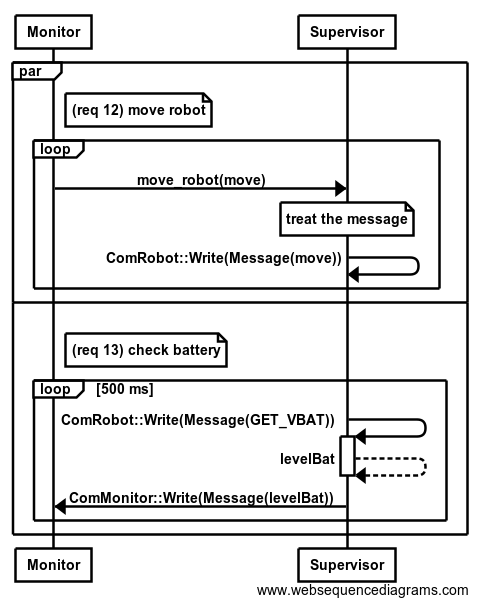
\includegraphics[scale=0.4]{./seq_req/req12-13}
\caption{Diagramme de séquence des fonctionnalités 12 et 13}
\label{fig:diag12_13}
\end{center}
\end{figure}
\FloatBarrier

%%%%%%%%%%%%%%%%%%%%%%%%%
\subsubsection{Gestion de la caméra}
%%%%%%%%%%%%%%%%%%%%%%%%%

Les fonctions permettant la manipulation des images sont fournies dans les librairies {\tt img} et {\tt camera}. L'implémentation des méthodes utilise \textsc{openCV}, une libraire libre en C/C++ de traitement d'images.

%%%%%%%%%%%%%%%%%%%%%%%%%
\paragraph{Ouverture de la caméra.} La méthode {\tt Open} de la classe {\tt Camera} donne accès à la caméra.\\

\req{La caméra doit être démarrée suite à une demande provenant du moniteur. Si l'ouverture de la  caméra a échoué, il faut envoyer un message au moniteur.}

%%%%%%%%%%%%%%%%%%%%%%%%%
\paragraph{Capture d'une image (mode nominal).} La méthode {\tt Grab} de {\tt Camera} permet de capturer une image. L'envoi de l'image au moniteur s'effectue normalement par l'envoi d'un message\footnote{L'image est compressée lors de l'envoi du message.}. La fréquence de capture d'une image est fixée par un paramètre lors de l'instanciation d'un objet {\tt Camera}.\\

\req{Dès que la caméra est ouverte, une image doit être envoyée au moniteur toutes les 100 ms.}

%%%%%%%%%%%%%%%%%%%%%%%%%
\paragraph{Fermeture de la caméra.} La méthode {\tt Close} de la classe {\tt Camera} permet de fermer proprement la caméra.\\

\req{La caméra doit être fermée suite à une demande provenant du moniteur. Un message doit être envoyé au moniteur pour signifier l'acquittement de la demande. L'envoi périodique des images doit alors être stoppé.}

%note right of Monitor
%(req 14) open camera
%end note
%Monitor->Supervisor: open camera
%Supervisor->+Supervisor: Camera::Open()
%Supervisor-->-Supervisor: err
%note over Monitor, Supervisor: ack or no_ack
%par
%loop camera active
%note right of Monitor
%(req 15) capture image
%end note
%Supervisor->+Supervisor: Camera:Grab()
%Supervisor-->-Supervisor: image
%Supervisor->+Supervisor: Img::ToJpg(image)
%Supervisor-->-Supervisor: jpgimage
%Supervisor->Monitor:ComMonitor::Write(Message(jpgimage))
%end
%else
%    note right of Monitor
%    (req 16) close camera
%    end note
%    Monitor->Supervisor: close camera
%    Supervisor->+Supervisor: Camera::Close()
%    Supervisor-->-Supervisor: err
%    note over Monitor, Supervisor: ack or no_ack
%end

\begin{figure}[htbp]
\begin{center}
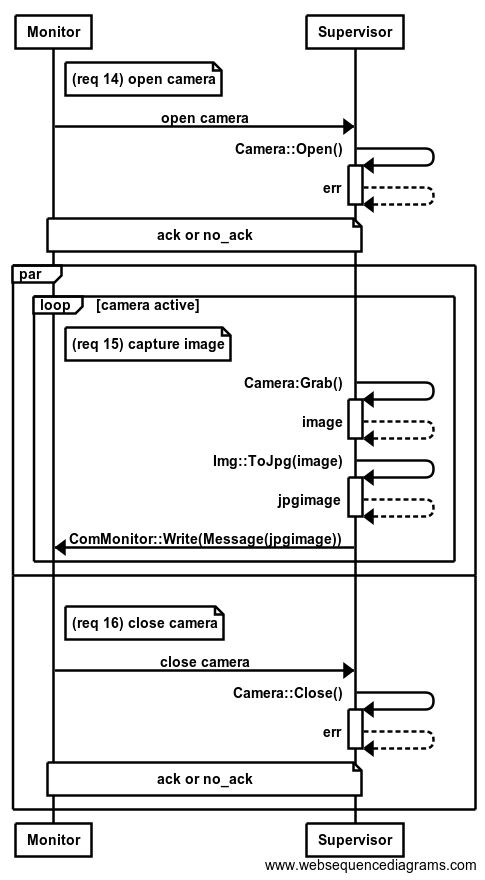
\includegraphics[scale=0.4]{./seq_req/req14-16}
\caption{Diagramme de séquence des fonctionnalités 14 et 16}
\label{fig:diag14_15}
\end{center}
\end{figure}
\FloatBarrier

\paragraph{Calibration de l'arène} Pour accélérer le traitement de l'image et le rendre plus stable\footnote{Si vous placez un robot en dehors de l'arène, il y a de fortes chances pour que cela perturbe le calcul de la position du robot.}, il est préférable de limiter la zone d'étude à l'arène. Pour cela il est nécessaire de faire un pré-traitement qui recherche l'arène.
 
Le calcul se fait par l'appel à la méthode {\tt SearchArena} de {\tt Img}. Il est possible de tracer sur l'image l'arène en faisant appel à la méthode {\tt DrawArena}.\\

\req{Suite à une demande de recherche de l'arène, le superviseur doit stopper l'envoi périodique des images, faire la recherche de l'arène et renvoyer une image sur laquelle est dessinée cette arène. Si aucune arène n'est trouvée un message d'échec est envoyé.\\

L'utilisateur doit ensuite valider visuellement via le moniteur si l'arène a bien été trouvée. L'utilisateur peut :
\begin{itemize}
	\item valider l'arène : dans ce cas, le superviseur doit sauvegarder l'arène trouvée (pour l'utiliser ultérieurement) puis retourner dans son mode d'envoi périodique des images en ajoutant à l'image l'arène dessinée.
 	\item annuler la recherche : dans ce cas, le superviseur doit simplement retourner dans son mode d'envoi périodique des images et invalider la recherche.
\end{itemize}
}

%note left of Monitor:(req 17) find arena
%Monitor->Supervisor:find arena
%note over Supervisor:stop periodic image
%Supervisor->+Supervisor: Camera:Grab()
%Supervisor-->-Supervisor: image
%Supervisor->+Supervisor: Img::SearchArena(image)
%Supervisor-->-Supervisor: arena
%alt arena == NULL
%Supervisor->Monitor:ComMonitor::Write(Message(NO_ACK))
%else
%Supervisor->+Supervisor: Img::DrawArena(image, arena)
%Supervisor-->-Supervisor: image
%Supervisor->+Supervisor: Img::ToJpg(image)
%Supervisor-->-Supervisor: jpgimage
%Supervisor->Monitor:ComMonitor::Write(Message(jpgimage))
%alt 
%    Monitor->Supervisor: arena ok
%    note over Supervisor: save arena
%else
%    Monitor->Supervisor: arena ko
%    note over Supervisor: delete arena
%end
%end 
%
%note over Supervisor: restart periodic image

\begin{figure}[htbp]
\begin{center}
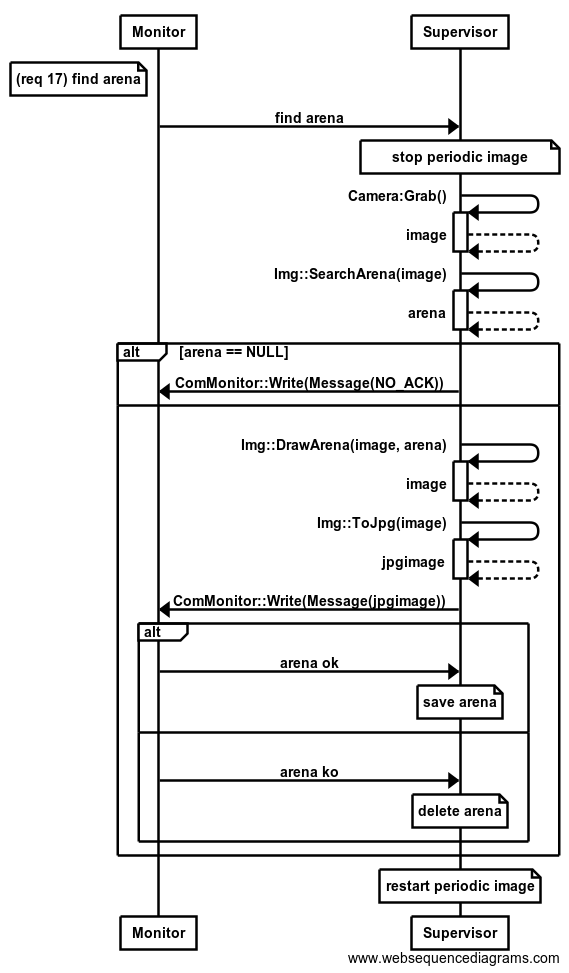
\includegraphics[scale=0.4]{./seq_req/req17}
\caption{Diagramme de séquence de la fonctionnalité 17}
\label{fig:diag16}
\end{center}
\end{figure}
\FloatBarrier

%%%%%%%%%%%%%
\paragraph{Calcul de la position du robot.} Le traitement d'une image pour trouver la position du robot se fait à l'aide de la méthode {\tt SearchRobot} de {\tt Img}. Il est possible de dessiner sur l'image la position trouvée en faisant appel à la méthode {\tt DrawRobot}. La position est envoyée du superviseur vers le moniteur en utilisant un message avec une entête dédié.\\
 
\req{Suite à une demande de l'utilisateur de calculer la position du robot, le superviseur doit calculer cette position, dessiner sur l'image le résultat et envoyer un message au moniteur avec la position toutes les 100~ms. Si le robot n'a pas été trouvé, un message de position est envoyé avec une position (-1,-1).}

%%%%%%%%%%%%%
\paragraph{Stopper le calcul de la position du robot.} Il est possible pour l'utilisateur de demander l'arrêt du calcul de la position.\\
 
\req{Suite à une demande de l'utilisateur de stopper le calcul de la position du robot, le superviseur doit rebasculer dans un mode d'envoi de l'image sans le calcul de la position.}
 
% note right of Monitor:(req 18) compute position
%Monitor->Supervisor:find_position
%loop
%Supervisor->+Supervisor: Camera:Grab()
%Supervisor-->-Supervisor: image
%Supervisor->+Supervisor: Img::SearchRobot(image, arena)
%Supervisor-->-Supervisor: position
%alt position != null
%    Supervisor->+Supervisor: Img::DrawRobot(image, positin)
%    Supervisor-->-Supervisor: image
%    Supervisor->Monitor:ComMonitor::Write(Message(position))
%else
%    Supervisor->Monitor:ComMonitor::Write(Message(position nulle))
%end
%    Supervisor->+Supervisor: Img::ToJpg(image)
%    Supervisor-->-Supervisor: jpgimage
%    Supervisor->Monitor:ComMonitor::Write(Message(image))
%end

 \begin{figure}[htbp]
\begin{center}
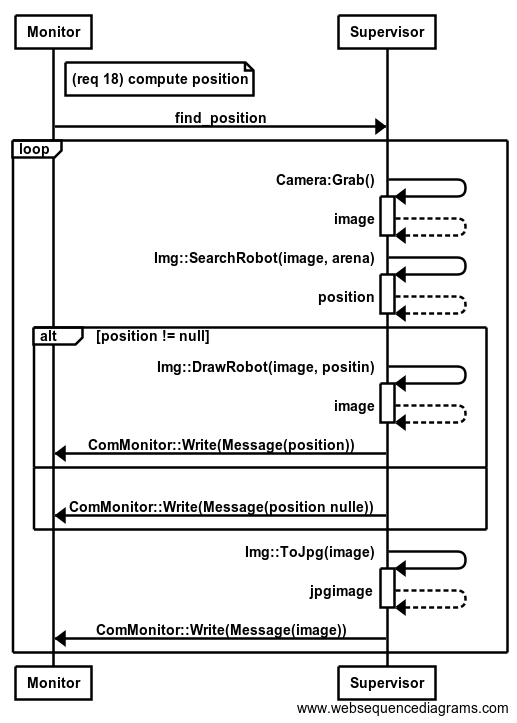
\includegraphics[scale=0.4]{./seq_req/req18}
\caption{Diagramme de séquence de la fonctionnalité 18}
\label{fig:diag17}
\end{center}
\end{figure}
\FloatBarrier
 
%%%%%%%%%%%%%%%%%%%%%%%%%%
\subsubsection{Réaliser une mission}
%%%%%%%%%%%%%%%%%%%%%%%%%%

TBD 
%Les missions à effectuer consistent  à déplacer le robot d'une position à une autre. Le choix de la destination se fait par l'utilisateur en cliquant sur l'image du moniteur puis en envoyant un message de type mission en la validant avec le bouton\og send mission \fg.
%
%Une mission est constituée de différents champs décrits dans un objet \texttt{DMission}. La position à atteindre peut être récupérée à l'aide de la méthode \texttt{d\_mission\_get\_position}. De plus, une mission est identifiée par un numéro contenu dans son champ \texttt{id}.
%
%La réalisation d'une mission s'effectue à l'aide des méthodes \texttt{d\_robot\_move} et \texttt{d\_robot\_turn}. Quand le point final est atteint, le superviseur doit envoyer un message de type mission portant l'identifiant de la mission. La méthode {\tt d\_message\_mission\_terminate} permet de construire un message portant les valeurs appropriées.
%
%Il est aussi possible pour l'utilisateur de mettre fin à une mission en cours en envoyant un message d'alerte (bouton \og Stop mission \fg). Ce message est de type {\tt MESSAGE\_TYPE\_MISSION} et porte \texttt{MISSION\_TYPE\_STOP} comme valeur dans le champ type. Dans ce cas le robot doit immédiatement s'arrêter puis le superviseur doit envoyer un message de fin de mission.
%
%Le diagramme~\ref{diag:seq_position} donne un aperçu de cette séquence.\\
%
%  \noindent\fcolorbox{black}{Fond}{%                couleur du texte, couleur du fond
%\begin{minipage}{\textwidth}
%Réaliser la fonction qui permet d'effectuer une mission. Aucune méthode n'est fournie pour concevoir le déplacement, le plus simple étant de tourner le robot dans la direction du point à atteindre puis d'avancer de la distance souhaitée.
%\end{minipage}
%}
